\documentclass[conference]{IEEEtran}
\usepackage{amsmath,epsfig}
\usepackage{graphicx}
\usepackage{epsfig,latexsym}
\usepackage{amsmath,amsfonts,amssymb,color}
\usepackage{graphicx}
\usepackage{subfigure}
\usepackage{multirow}
\usepackage{bbm}
\usepackage[T1]{fontenc}
\usepackage{url}
\renewcommand{\textfraction}{.01}
\renewcommand{\bottomfraction}{.99}
\renewcommand{\topfraction}{.99}

% correct bad hyphenation here
%\hyphenation{op-tical net-works semi-conduc-tor}


\begin{document}
%
% paper title
% can use linebreaks \\ within to get better formatting as desired
\title{Fireworks: Evolutionary art project based on EvoSpace-Interactive}


% author names and affiliations
% use a multiple column layout for up to three different
% affiliations

\author{\IEEEauthorblockN{Leonardo Trujillo\\ and Mario Garc\'ia-Valdez}
\IEEEauthorblockA{Divisi\'on de Estudios de Posgrado \\
Instituto Tecnol\'ogico de Tijuana, Mexico \\
Email: leonardo.trujillo@tectijuana.edu.mx \\
mario@tectijuana.edu.mx}
\and
\IEEEauthorblockN{Francisco Fern\'andez-de-Vega}
\IEEEauthorblockA{Grupo de Evoluci�n Artificial\\
Universidad de Extremadura, Spain\\
Email: fcofdez@unex.es}
\and
\IEEEauthorblockN{Juan-J. Merelo}
\IEEEauthorblockA{Departamento de Arquitectura y\\
Tecnolog\'ia de Computadores\\
University of Granada, Spain\\
Email: jmerelo@geneura.ugr.es}}

% make the title area
\maketitle


\begin{abstract}
This paper presents a collaborative-interactive evolutionary algorithm (C-IEA) that evolves artistic animations and is executed on the web.
The application is called \emph{Fireworks}, since the animations that are produced
are similar to an elaborate fireworks display.
The system is built using the EvoSpace platform for distributed and
asynchronous evolutionary algorithms.
EvoSpace provides a central repository for the evolving population and
remote clients, called EvoWorkers, that interact with the system to perform individual evaluation using and interactive approach.
The artistic animations are coded using the Processing programming
language that facilitates rapid development of computer graphics applications for artists and graphic designers.
The system promotes user collaboration and interaction by allowing many
users to participate in population evaluation and because the system incorporates social networking.
Initial results show that the proposed C-IEA can allow users to produce
interesting artistic artifacts that incorporate preferences from several
users, evolving dynamic animations that are unique within evolutionary art.
\end{abstract}

% IEEEtran.cls defaults to using nonbold math in the Abstract.
% This preserves the distinction between vectors and scalars. However,
% if the conference you are submitting to favors bold math in the abstract,
% then you can use LaTeX's standard command \boldmath at the very start
% of the abstract to achieve this. Many IEEE journals/conferences frown on
% math in the abstract anyway.

% no keywords
\begin{IEEEkeywords}
Distributed algorithms, cloud computing, interactive evolutionary algorithm, linear genetic programming.
\end{IEEEkeywords}



% For peer review papers, you can put extra information on the cover
% page as needed:
% \ifCLASSOPTIONpeerreview
% \begin{center} \bfseries EDICS Category: 3-BBND \end{center}
% \fi
%
% For peerreview papers, this IEEEtran command inserts a page break and
% creates the second title. It will be ignored for other modes.
\IEEEpeerreviewmaketitle

\section{Introduction}
Artificial evolution has proven to be a powerful computational paradigm used to solve optimization, search and learning problems in diverse domains.
Moreover, evolutionary algorithms (EAs) have found a wider application area than just traditional engineering or scientific domains,
with promising contributions to art, music and design being developed at a steady pace over recent years \cite{todd:1992,DBLP:conf/evoW/McCormack05,picbreeder,forms,evoeco}.
The nature of EAs, which combine a balanced mixture of exploitative optimization with explorative search, has allowed EAs to become robust and versatile
algorithms that solve difficult non-linear and discontinuos problems, even in cases where an analytic or automatic objective
function cannot be derived \cite{DBLP:books/daglib/0015527}.

In particular, when dealing with creative domains, fitness usually needs to incorporate some sort of human knowledge and preferences,
either off-line (before the search) or on-line (during the search). The former case are referred to as supervised learning algorithms,
while the latter case refers to interactive EAs (IEA).
Human interaction is required in these domains because creativity and aesthetic principles are not yet fully understood, which limits
the possibility of measuring them directly and objectively.
That is why researchers have turned towards humans to provide an indirect and subjective evaluation of evolved artistic artifacts.
While the IEA approach solves one problem, it also creates others, such as the following.
First, a human can easily get tired of what can be a monotonous task of evaluating many individuals over many generations,
most of which will only be marginally interesting.
Secondly, a user can get bored, and start to provide feedback that deviates from his original goal.
Finally, given the subjective nature of evaluating artistic design, a single user might not provide the required feedback;
i.e., the fitness landscape might not present the necessary structure for the search to proceed in a non-random way.
Nonetheless, IEAs have been used to generate impressive artistic designs,
incorporating insights from computer science and artificial intelligence researchers, as well as artists from various domains.

Only until recently, however, has an EA tool been proposed that is specifically aimed at IEA for artistic design.
EvoSpace-Interactive was developed with this goal in mind, providing a simplified development interface for IEAs \cite{evospace1,evospace2}.
Moreover, EvoSpace-Interactive was designed to incorporate and combine the subjective opinions from different users of the system.
EvoSpace-Interactive employs a cloud-based population manager that allows for asynchronous and distributed interaction from users, and employs social network integration to promote user collaboration and interaction.
Therefore, we shall refer to EvoSpace-Interactive as a Collaborative-IEA (C-IEA).

In \cite{evospace2} the EvoSpace tool is presented and in \cite{evospace1} a proof-of-concept implementation was presented for a C-IEA for artistic design.
In the present paper, on the other hand, the first advanced evolution of artistic artifacts using EvoSpace.
Moreover, the application exploits the Processing programming language, that
facilitates artistic development for non-computer scientists.
Moreover, the system incorporates and promotes user collaboration by integrating with a social networking service.
The proposed system is called \emph{Fireworks}, that employs a linear genetic programming (LGP) approach \cite{field} to evolve artistic animations
of particle swarms that visually resemble a fireworks display.

The remainder of this paper proceeds as follows.
First, Section \ref{sec:related} presents a discussion of related works.
Then, Section \ref{sec:evo} presents the EvoSpace platform for C-IEAs.
The \emph{Fireworks} system is described in Section \ref{sec:fire}, detailing
the LGP algorithm and Processing based representation of individuals.
Experimental results are summarized and discussed in Section \ref{sec:exp}.
Finally, Section \ref{sec:conclusions} outlines the main conclusions of the work.

\section{Related Work}
\label{sec:related}
The goal of IEAs is to use human preferences as the main (or only) source of selective pressure that guides an evolutionary search \cite{ie1,ie2}.
IEAs pose an open-ended search where the objective function used by traditional EAs is replaced by the subjective
preferences and interaction of human users of the system.
Indeed, some of the earliest EAs were open-ended systems, such as the well-known Biomorphs algorithm developed by Richard Dawkins\cite{biomorphs}.
Therefore, IEAs should encourage high diversity and exploration given the dynamic and non-deterministic nature of the evaluation process \cite{ns:2012}.

IEAs have been used in various domains and applications;
for instance, \cite{implant} uses an IEA to evolve medical implants to improve hearing.
However, the present work focuses on the evolution of artistic animations using a collaborative and distributed approach.
IEAs that incorporate user collaboration and interaction are here referred to as Collaborative-IEAs or C-IEAs;
some noteworthy works in this area are reviewed next.

An early example of a web based interactive system is the work by Langdon \cite{langdon:2004}, where fractal representations of virtual creatures were evolved.
He proposed a distributed EA using a global population that resides on a central website and uses Javascript to distribute
portions of the population to remote clients.
Users evaluate individuals locally and those a user prefers are returned to the server and can be distributed again to others,
thus promoting a collaborative process during evolution.
Similarly, Secretan et al. \cite{picbreeder} and Clune and Lipson \cite{forms} use web-based IEAs to evolve artistic artifacts
using compositional pattern producing networks as a generative encoding.
In \cite{picbreeder} images are evolved, while 3-D sculptures are evolved in \cite{forms}.
In both cases, users (connected clients) are encouraged to collaborate.
In both works a central websites was developed where users can select or create random individuals and evolve lineages of artifacts based on their preferences.
In these systems a user can take a previously evolved artifact and continue the search process himself, building upon earlier design in a sequential
manner.
Therefore, the evolved artifacts can be the product of a collaborative evolutionary search.
Another feature is that evolved artifacts can be rated by users, and given that users can create individual accounts, the ratings provide a way to rank users,
or to select previously evolved artifacts based on the particular style of each user.
Furthermore, the collaborative process is captured by the system, since it is possible to visualize how, and when, different users influenced
a genetic lineage.
Kowaliw et al. \cite{evoeco} present recent example based on evolving ecosystemic models, a generative encoding based on multi-agent systems
that generate high quality artistic drawings.
Again, users visit a website and interact with a Java applet,
after which they can choose to add evolved images to a central collection such that other users can see them or them as seeds for their own evolutionary design.


The present work builds on previous proposals and extends the C-IEA approach.
First, it promotes collaborative evaluations of artistic artifacts in a dynamic and parallel manner,
instead of the sequential approach followed in \cite{picbreeder,forms}.
Second, it incorporates explicit user interactions by encouraging the use of social networking.
Third, by exploiting the Processing programming language for graphics programming, it facilitates rapid development for artists
with a limited computer science background.
Fourth, it focuses on the evolution of artistic animations, not static pictures or paintings; another feature facilitated by the use of Processing.
Fifth, it facilitates the ability to save and share promising artifacts.
Finally, it emphasizes the use of a distributed model, to exploit current trends in software and hardware technology.

\section{EvoSpace}
\label{sec:evo}
EvoSpace is a population store for the development of evolutionary algorithms that are intended to run on a cloud computing model \cite{evospace2}.
It is designed to be versatile, since the population is decoupled from any particular evolutionary algorithm.
Client processes, called EvoWorkers, dynamically and asynchronously interact with the EvoSpace store and perform the basic
routines of an evolutionary search.
EvoWorkers can reside on remote clients or on the platform server itself.
The EvoSpace platform is presented in \cite{evospace2}, here we only provide a general outline of how the system functions.

EvoSpace consists of two main components.
The first one is the EvoSpace container, used to store the EA population.
The second component consists of the remote clients or EvoWorkers, which
execute the actual evolutionary process.
Figure \ref{fig:evo} presents a schematic diagram of the EvoSpace system and data flow.

\begin{figure*}[t]
    \centering
        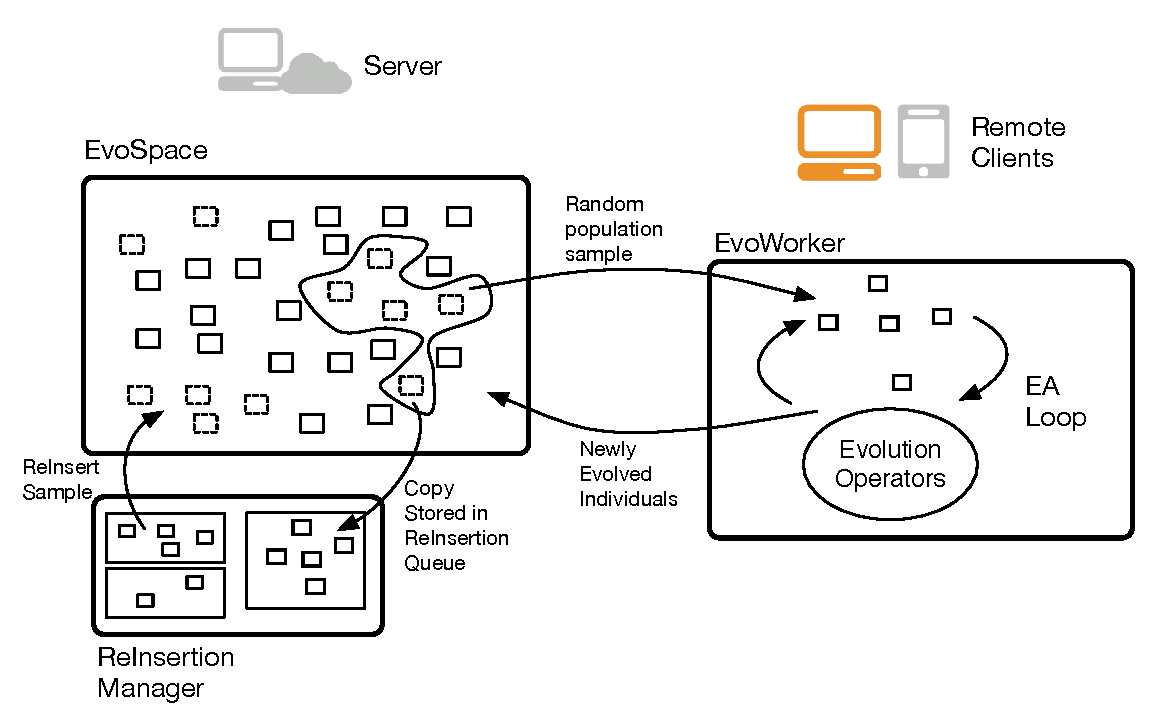
\includegraphics[width=14cm]{evospaceExample.eps}
    \caption{Main components and dataflow within the EvoSpace platform. The figure illustrates the two main components, the EvoSpace container on the server and the remote
    EvoWorker clients. Notice how the population is samples and distributed to the clients where evaluation and other evolutionary operators can be applied.}
    \label{fig:evo}
\end{figure*}



\subsection{The EvoSpace container.}
EvoSpace is based on the tuplespace model, a distributed shared memory (DSM) abstraction organized as a \emph{bag} of tuples.
A tuple $t$ is the basic tuplespace element, composed by one or more fields and corresponding values.
In this model the basic operations that a process can perform is to insert or withdraw tuples from the tuplespace.
EvoSpace is composed by a set of objects $ES$ and a set of interface methods provided by a central server.
The current EvoSpace implementation offers the following interface methods ti withdraw and replace objects from $ES$.

\textbf{Read(n):} This method returns a random set $A$ of objects from $ES$, with $|A|=n$ and $A\subset ES$, if $n< |ES|$, the method returns $ES$ otherwise.

\textbf{Take(n):} Returns a random set $A$, following the similar logic used for $Read()$.
However, in this case the sequence of $Take()$ operations provide a temporal dimension to the dynamics of set $ES$.
We can define $ES_i$ as the set at the moment of the $i-th$ $Take()$ operation and $A_i$ as the output.
The contents of EvoSapce are then given by $ES_{i+1}= ES_i \setminus A_i$; i.e., the objets taken are effectively removed from $ES$.
The objects taken are also copied to a new set $S_i$ of \emph{sampled objects} and stored
within a temporary collection $\mathcal{S}$ on the server, implemented as a priority queue.
Sets $S_i \in \mathcal{S}$ can then be reinserted to $ES$ if necessary.

\textbf{ReInsert(i):} This method is used to reinsert the subset of elements removed by the $i-th$ $Take()$ operation,
  such that the contents of EvoSpace are now $ES \cup S_i$ if $S_i \in \mathcal{S}$ and $ES$ is left unchanged otherwise.

\textbf{Insert(A):} This method represents the union operation $ES \cup A$.

\textbf{Replace(A,i):} Similar to $Add()$, however set $A$ should be understood as a replacement for
  some $S_i \in \mathcal{S}$, hence $|A| = |S_i|$, but the objects in $A$ can be different (evolved) objects from those in $S_i$.
  Moreover, if $S_i$ exists it is removed from $\mathcal{S}$.
  However, if $S_i$ does not exist this means that a $ReInsert(i)$ operation preceded it, this increases the size of $ES$.

\textbf{Remove(A):} This method removes all of the objects in $A$ that are also in $ES$, in such a way that
  the contents of EvoSpace are now set to $ES \cup (A\cap ES)$.

The sub-components of EvoSpace are summarized below.

\emph{Individuals.}
The objects contained within $ES$ represent the evolving individuals of an EA.
Individuals in $ES$ are stored as \emph{dictionaries}, a collection of unique keys and values with a one to one association.


\emph{The EvoSpace Server.}
On the server side the \texttt{EvoSpaceServer} process creates and activates a new EvoSpace
container object and waits for requests to execute interface methods.
Three other server processes are also executed: \texttt{InitPopulation}, \texttt{ReInsertionMgr} and \texttt{EvolutionMgr}.
\texttt{InitPopulation} initializes the population with a total of $popsize$ random individuals.
\texttt{ReInsertionMgr} periodically checks (every $wt$ seconds) if the size of the population in $ES$
falls below a certain threshold $min$ or if the time after the last reinsetion is greater than $next_r$.
If any of these conditions are satisfied, then $rn$ subsets $S_i \in \mathcal{S}$ are reinserted into ES using the $ReInsertOld()$ method.
Finally, \texttt{EvolutionMgr} periodically checks if a termination condition is satisfied according to the needs of the evolutionary search.
For an open-ended C-IEA a termination criteria is usually not implemented, and is left up to the researcher to halt evolution when he consideres it necessary.



\emph{EvoWorkers.}
The \texttt{EvoWorker} process requests a set of $ew_{take}$ individuals from the $ES$ container using the $Take()$ interface method provided by EvoSpace.
In the case of an IEA, the individuals are presented to a user of the system which is prompted to evaluate them.


\emph{Evolve Process.}
Finally, in the case of an C-IEA, after a pre-specified number of $Take()$ operations $evolve_{threshold}$ the $Evolve()$ function is invoked on the server side,
which proceeds to request a set of $ev_{take}$ individuals using the $Take()$ method, on which the specified set of genetic operators (selection, mutation, crossover, etc.)
are applied to generate offspring which are then returned and reinserted into the population.

\emph{Implementation of the population store.}
Individuals are stored in-memory, using the Redis key-value database.
Redis was chosen over a SQL-based management system, or other non-SQL alternatives,
because it provides a hash based implementation of sets and queues which are natural data structures for the EvoSpace model.
For example, selecting a random key from a set has a complexity of O(1).
The logic of EvoSpace is implemented as a Python module exposed as a Web Service using cherrypy and Django HTTP frameworks.
The EvoSpace web service can interact with any language supporting json-rpc or ajax requests.
The EvoSpace modules and workers in JavaScript, JQuery and python are available with a Simplified BSD License from \url{http://evospace.org}.

\subsection{EvoSpace-Interactive.}
This paper presents a C-IEA system based on an extension of the EvoSpace platform called EvoSpace-Interactive \cite{evospace1},
depicted in the block diagram of Figure \ref{fig:CIE}.
With EvoSpace-Interactive developers can exploit a platform for distributed user collaboration and interactive evolution
that offers the following:
a central repository for the population implemented as an EvoSpace service;
a Web Application script implemented using Django; and a mature full stack Web Framework with a BSD license developed in Python.
EvoSpace-Interactive is responsible for user authentication and session handling through the popular Facebook social network using the OAuth 2.0 protocol.
Also, the storage of collections, where users can store individuals they want to share with friends, is persisted using the PostgreSQL DBMS.
Most of the interactive functionality is programmed in the client side using Javascript libraries.
The communication between components is implemented using json-rpc, a lightweight remote procedure call protocol and common ajax and http transactions.
Overall functionality is decomposed in specialized services, adding flexibility to the framework since services can be interchanged.
The framework is built using only open source components from libraries to servers.
Users interact with the system through a GUI implemented on a Responsive Web Design (RWD) front end framework,
an approach to web design in which a graphical user interface is crafted to provide a satisfactory viewing experience in a range of mobile devices.
This approach enables designers to tailor the look and feel of the application with minimum intrusion, only changing CSS definitions.

Three components must be specified by the application developer, marked with double lines in Figure \ref{fig:CIE}; these are:
an \emph{individual} representation; a \emph{processing script} that renders each individual;
and a \emph{worker} script that encodes the evolutionary operators depending upon the proposed representation.
Each of these points are discussed below.

\begin{figure*}[t]
    \centering
        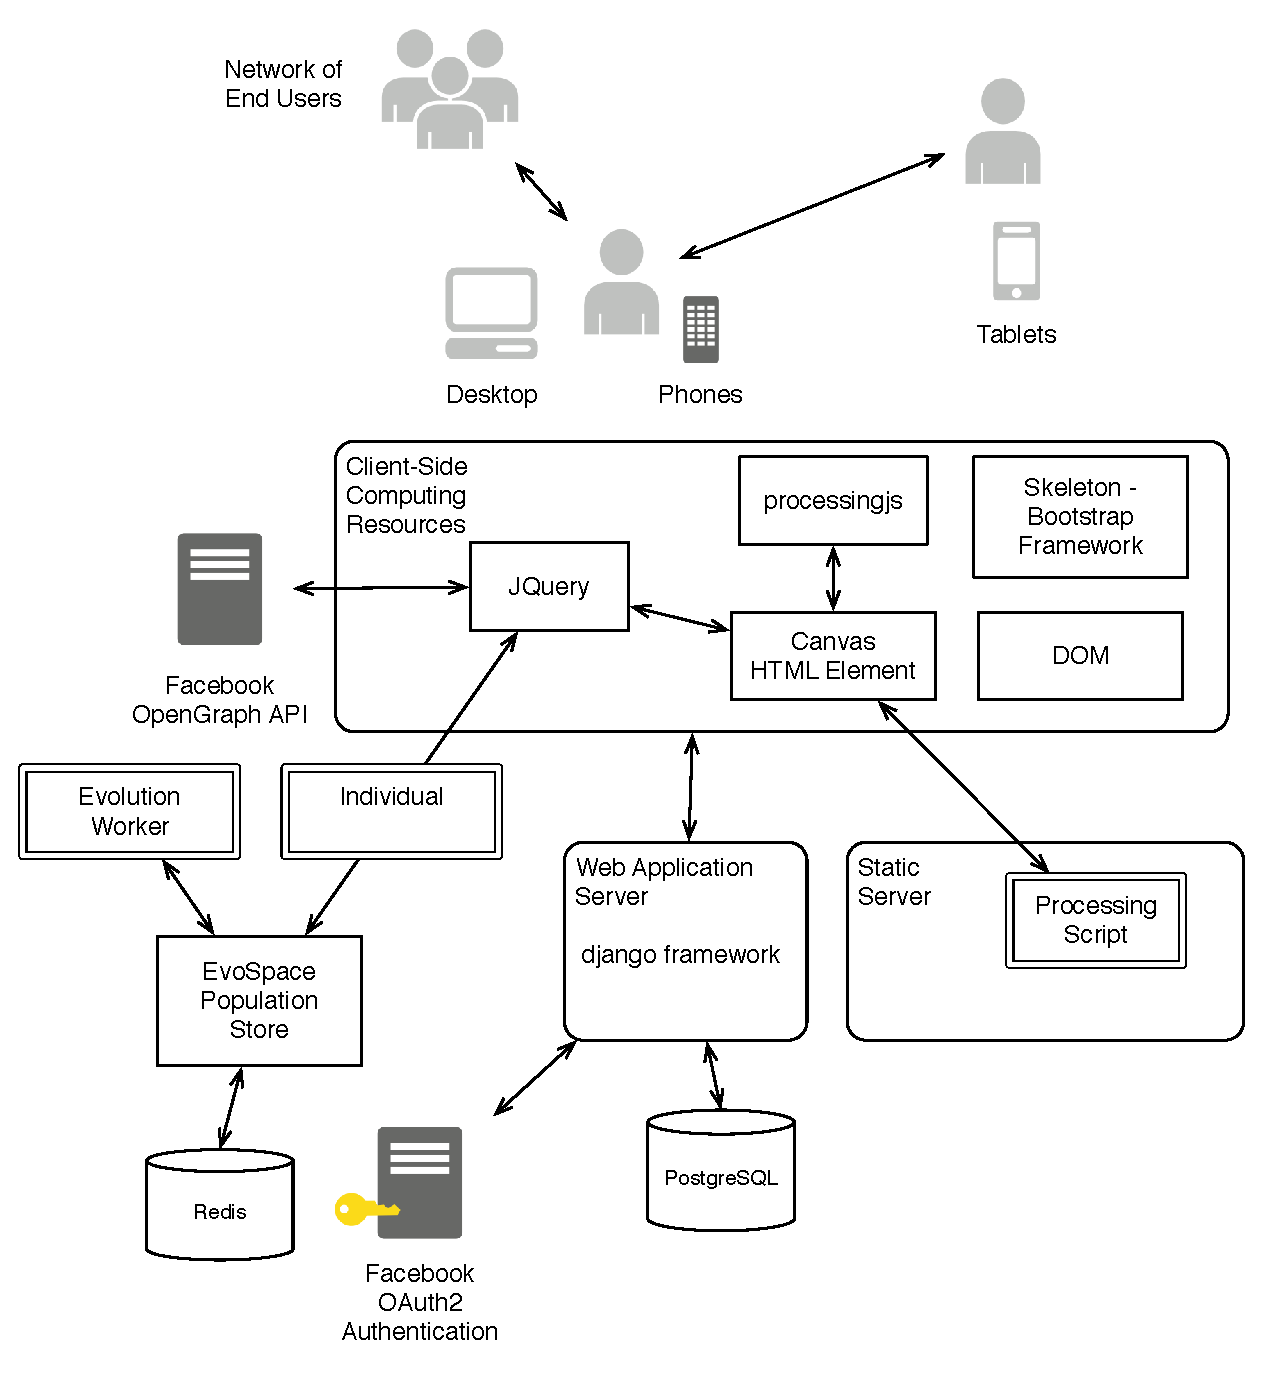
\includegraphics[width=14cm]{arq.eps}
    \caption{Conceptual design of the proposed C-IEA.
    The figure presents a block diagram of the main software components of the system and how they interact with each other on the cloud,
    to provide a collaborative interactive application for remote client users.}
    \label{fig:CIE}
\end{figure*}




\subsection{User Interface}
The users interact with the web interface composed of the five elements proposed in \cite{evospace1}, see Figure \ref{fig:web}.
First, at the top left corner user login, where users can link to their Facebook account or decide to participate as an anonymous user.
Second, to encourage user interaction when a user chooses to login to his Facebook account a list of friends that have also linked
to the C-IEA application is presented on the left.

\begin{figure*}[t]
    \centering
        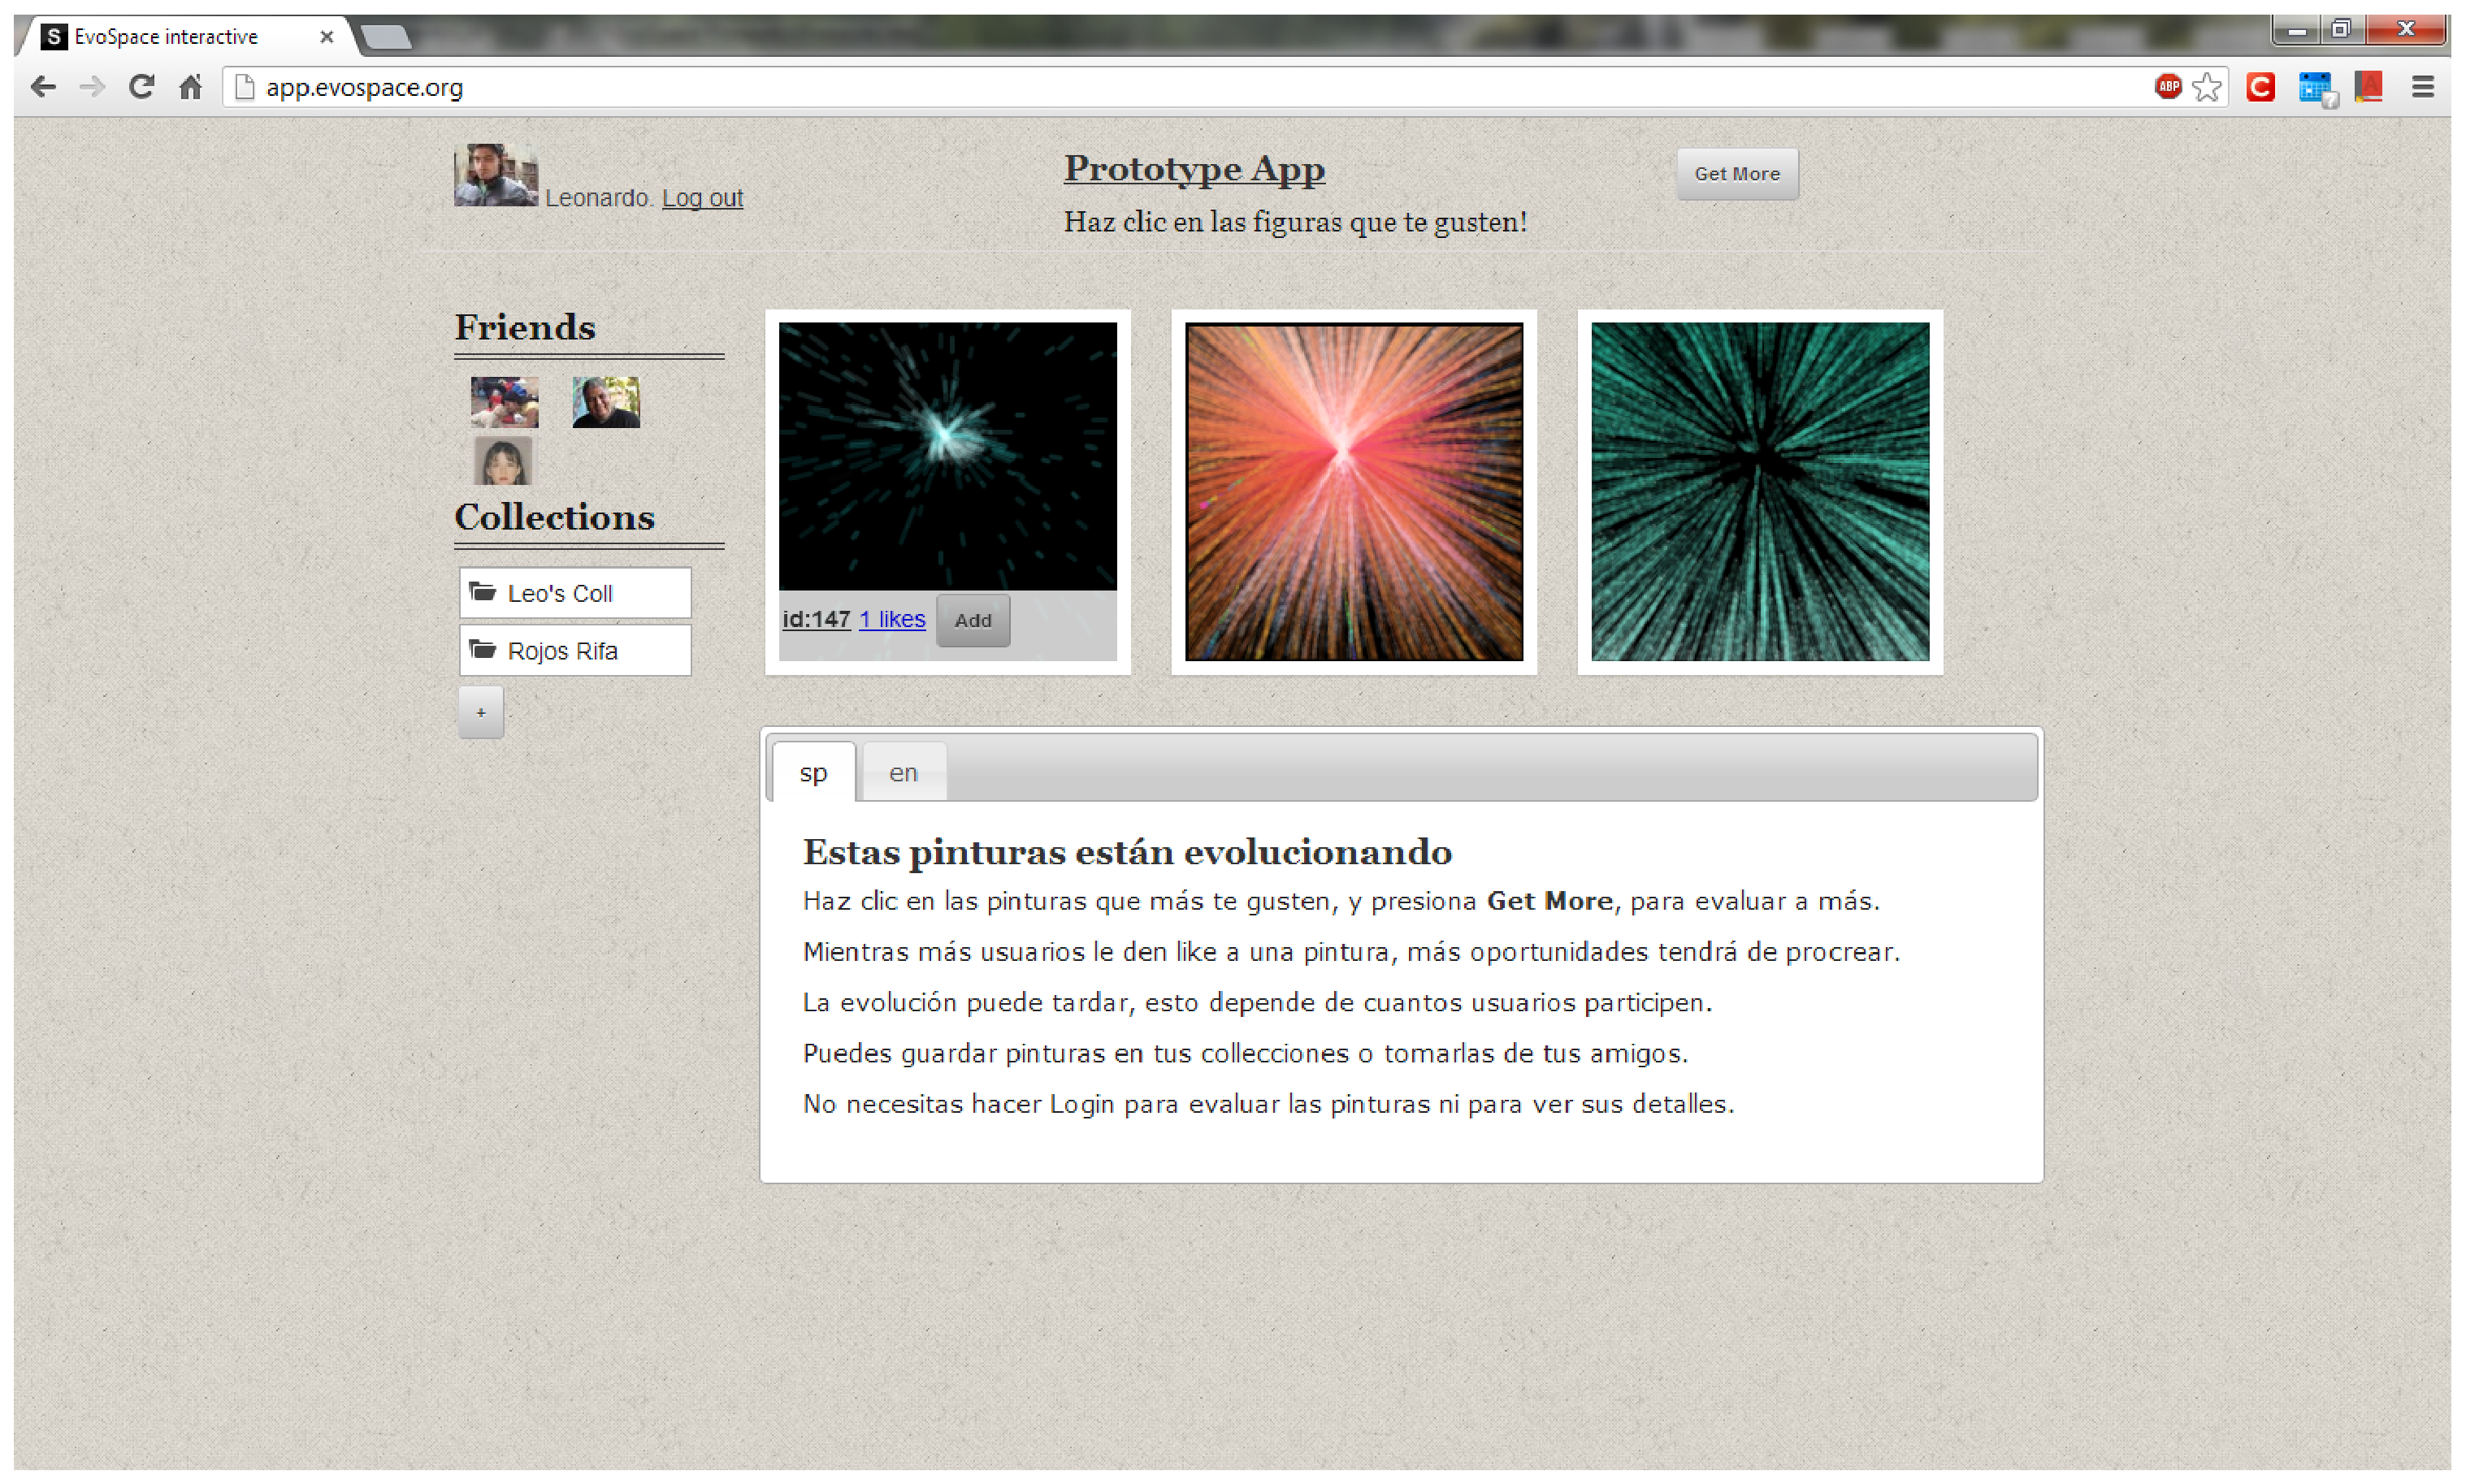
\includegraphics[width=12cm]{EvoApp.eps}
    \caption{User interface of the EvoApp C-IEA.}
    \label{fig:web}
\end{figure*}

The third element is a central \emph{Wall} area, where $ew_{take}$ randomly sampled individuals by a $Take()$ operation are shown to the user.
Here, the user can interact with the system by clicking on the individuals he prefers, which counts as a ''like" for the individual,
or the user can add an image to a \emph{collection} of individuals, a special directory to store individuals a user prefers and wishes to save.

After the user finishes interacting with the current crop of individuals he can choose to retrieve a new sample from EvoSpace.
This is done with the fourth element of the interface, located at the top of the screen, the \emph{Get More} button.
The button returns the current group of individuals to EvoSpace, and brings back a new one.

The \emph{collections} section is the fifth element of the interface, shown at the bottom left corner.
The user can create as many collections as he wants to organized his preferred individuals.
Moreover, a user can browse the content of each collection and from there share images through the social network.
When a user browses over an individual a detail pane shows the list of users that have liked the individual.

\subsection{Individual Representation}
As stated above, individuals are represented internally as a dictionary.
The properties stored by EvoSapce-Interactive applications are: a unique \texttt{id}; a user defined \texttt{chromosome};
the number of times the individual has been selected in a sample and returned to the population, stored in property called \texttt{views};
the genetic operators that generated the individual; ids of the parents; \texttt{current Fitness} that stores the most resent fitness value;
and a \texttt{fitness} dictionary where each key is a concatenation of a \texttt{userid}, a \texttt{timestamp} and a numerical value that represents
the rating given by the corresponding individual.
A UML representation of an individual is presented in Figure \ref{fig:individual}.


\begin{figure}[t]
    \centering
        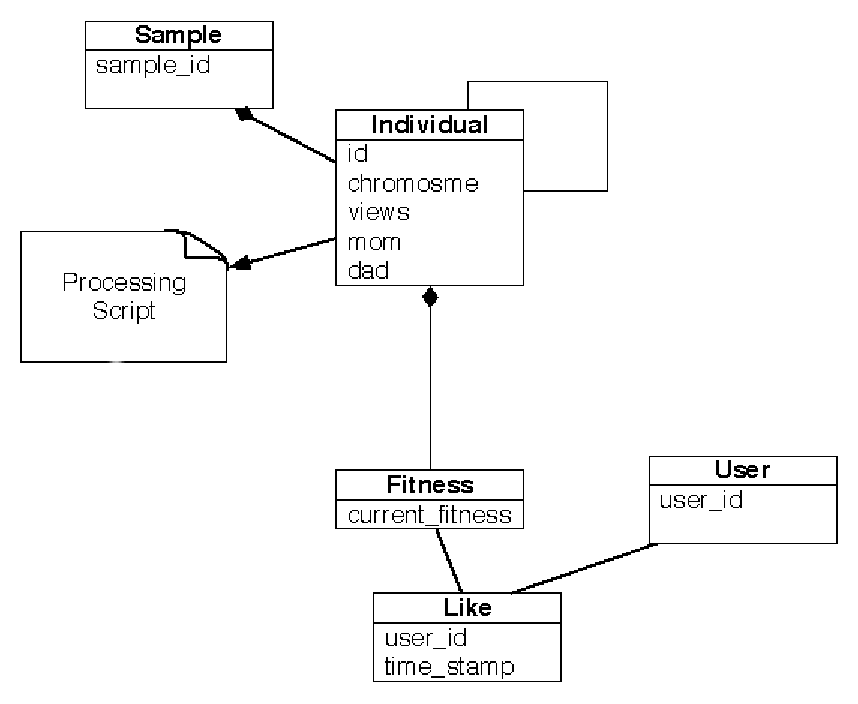
\includegraphics[width=8cm]{UMLIndividual.eps}
    \caption{Individual internal representation.}
    \label{fig:individual}
\end{figure}

\subsection{Processing Language and HTML Canvas Element}
Processing is a programming language and development environment initially created to serve as a software sketchbook and as a tool to teach fundamentals
of computer programming within a visual context.
Currently is used by artists, designers, architects, and researchers for visualization applications, games and interactive animations projects \cite{Reas:2007wp}.
Processing is a subset of Java directed to novice programmers and generative artists \cite{Pearson:2011ti}, which are the intended users of the
EvoSpace-Interactive framework.
As a complement there is a javascript library \emph{processingjs} that allows Processing scripts to be run by any HTML5 compatible browser.
Processing scripts are render individuals on the web interface, which can involve static images, animations, sound or even interactive artifacts.
Before calling the $draw()$ method of the processing script initial place holding or fallback parameters are replaced with an individual's chromosome.
Each individual's script has its own Canvas entity, defined by the HTML5 standard as an element that provides scripts with a resolution-dependent bitmap canvas
which can be used for rendering graphics on the fly.
Although the combination of an HTML5 Canvas element and a Processing script is supported by default, other combinations could be used.
For instance, images, embedded audio, or other libraries capable of drawing in the Canvas.
Also, a fallback implementation must be considered for applications intended for non-HTML5 capable browsers.

\section{Fireworks Application}
\label{sec:fire}
This section presents the evolutionary art application proposed in this work called Fireworks.
First, the artistic artifacts are described, developed using Processing scripts that can produce complex graphics in a simple development language.
Afterwards, the linear GP encoding of individuals is given.
Finally, the genetic operators for selection, crossover and mutation are described, as well as the fitness assignment process.

\subsection{Fireworks Swarm Animations}
The goal of the Fireworks C-IEA is to evolve artistic animations of particle swarms.
It is noteworthy to point out that evolving animations is a unique application within current evolutionary art literature that mostly focuses on static images or sculptures.
The animations are based on the open-source Processing script developed by Claudio Gonzales called Galactic Dust
available at \url{http://www.openprocessing.org/sketch/8062}, licensed under Creative Commons Attribution-Share Alike 3.0
\footnote{\url{ttp://creativecommons.org/licenses/by-sa/3.0/}} and GNU GPL license\footnote{\url{http://creativecommons.org/licenses/GPL/2.0/}}.
The Galactic Dust script presents a virtual 3D canvas where a set of $N$ particles can move about.
In the original version of the script the particles are randomly positioned within the 3D canvas (or placed in an a priori pattern) and remain static.
Then, when the user left-clicks on a point within the canvas this specifies the position of a gravitational point $P$ on the canvas
and produces an attractive force on all of the particles towards $P$, proportional to their distance to $P$ and mass which is also specified initially.
Similarly, when a user right-clicks on the canvas a repulsive force is produced.
Moreover, the particles continuously change color using small random steps and the user can toggle
a tracing effect on or off, in which each particle leaves a visual trail of its movements that gradually disappears with time.

The Galactic Dust script is the inspiration and basis for the artistic animations evolved by the Fireworks application.
In particular, the goal of Fireworks is to begin with randomly placed particles and to evolve a pattern of movements and
behaviors, searching for interesting visual animations.
These animations are similar to popular screensavers or background visualizations for music players,
however the authors feel that an illustrative description is to say that they resemble elaborate fireworks displays, thus the name.
In the following subsection, the search space representation is described.


\subsection{Linear Genetic Programming Representation}
The C-IEA uses a LGP representation \cite{field} for the evolution of the Fireworks' swarm animations.
Initially, all individuals begin with the central pixel of the 3D canvas as the gravitational point $P$.
The chromosome of each individual is encoded as a variable-length list.
Each element, or gene, of the chromosome represents one of five basic operations, these are: $Attract_{flag}$, $Move_{flag}$, $Trace_{flag}$,
$ForwardX_{flag}$, $ForwardY_{flag}$  and $Step_m$.
The first four instructions are toggle operations for different
script parameters that determine the characteristics of particle movements.
$Attract_{flag}$ instructs the script to toggle between attraction or repulsion towards $P$.
$Move_{flag}$ toggles between particle movement or particle deceleration at each frame of the animation.
$Trace_{flag}$ determines if particle movement will produce tracing or if it will not.
$ForwardX_{flag}$ and $ForwardY_{flag}$ flags determines the orientation of particle movements in the horizontal and vertical axis respectively.
Finally, the $Step_m$ function determines the magnitude of step movements in each direction given by $m$ pixels, with a random decision uniformly
chooses from $u \in [1,13]$.



\subsection{Genetic Operators}
The LGP search employs several types of genetic operators.
Firstly, two crossovers are implemented: $2pCross$ and $appendCross$.
$2pCross$ chooses two random crossover points on each parent separately and swaps the corresponding sublists between the parents, generating two offspring.
If the sublists are of different size then one of the offspring will increase in size while the size of the other will decrease.
$appendCross$ produces two offspring that are the concatenation of both parent chromosomes, each in different order.
Secondly, five mutation operators are implemented: $Shuffle$, $Move$, $Delete$, $Replace$ and $Insert$.
The $Shuffle$ mutation randomly permutates the genes in a parent chromosome.
The $Move$ mutation randomly selects a chromosome sublist and then moves it to a new random position within the parent chromosome.
The $Delete$ mutation randomly selects and deletes a sublist from the parent chromosome.
The $Replace$ mutation randomly selects and deletes a sublist from the parent chromosome and replaces it by a new random list.
Finally, $Insert$ mutation generates a new list and splices it into a randomly chosen position within the parent chromosome.

The C-IEA uses tournaments for parent selection, and a crossover and mutation rate determines whether or not the genetic operators are applied.
Crossover is applied first and then the resulting offspring are mutated.
The crossover and mutation operator that is actually applied is chosen uniformly at random for each pair of parents.
The survival strategy is a steady-state implementation, where the offspring generated by the genetic operators
replace the two worst individuals from the selection tournament.

\begin{table*}[t]
\caption{Parameters of the C-IEA used by the \emph{Fireworks} application.}
\centering
\begin{tabular}{|l|c|}
\hline
 {\bf Parameter}                                                   & {\bf Value}  \\
\hline
 \textit{Population size}                                          & 100 individuals\\
\hline
\textit{Sample size taken by EvoWorkers $ew_{take}$ }              & 3 individuals\\
\hline
\textit{Number of samples before $Evolve()$ process $ev_{take}$}   & 10 samples\\
\hline
\textit{Tournament size of the $Evolve()$ process}                 & 6 \\
\hline
\textit{Number of offspring generated by the $Evolve()$ process}   & 2 \\
\hline
\textit{Survival}                                                  & Elitist steady-state survival \\
\hline
\textit{Operator probabilities (crossover and mutation)}           & $p_c=1$ and $p_m=0.3$ \\
\hline
\end{tabular}
\label{tab:params}
\end{table*}

\subsection{Fitness Evaluation}
The fitness of each individual is computed based on the number of users who liked it relative to the number of times if has been seen.
In the current implementation, users can only give positive evaluations
explicitly when they select an individual, a \emph{like}.
However, the system also keeps track of the number of times an individual has been sent to an EvoWorker client for evaluation,
the \emph{views} property.
When a user evaluates a sample of individuals, some (or all) of them will not receive a vote, but in all cases
the \emph{views} property will be incremented by 1.
If an individual has a high number of \emph{views} with a relatively small number of \emph{likes}, then the individual is considered to be less fit
then an individual with basically the same number of \emph{views} and \emph{likes} if if the values are low.
In other words, the ratio $\frac{likes}{views}$ is more informative, but it
does not distinguish between an individual with many \emph{views} and another with
only one \emph{view} if they both have zero \emph{likes}.
Additionally, \emph{views} must be >=1 to avoid a division by zero.
Therefore, fitness is assigned based on $\frac{likes+1}{views+1}$.


\section{Experiments}
\label{sec:exp}
This section provides details regarding the experimental setup and the results obtained until now.
First, Table \ref{tab:params} summarizes the parameters of the C-IEA used by the \emph{Fireworks} application.
Currently, the \emph{Fireworks} applications has been evolving individuals for over one week,
progressively generating novel animations.
In general, it is clear that the genetic representation and evaluation criteria has allowed the algorithm
to progressively incorporate the preferences of several users.
There is no time-table to halt the open-ended evolutionary process, and the system is expected to run for at least one more month.
It is now possible to access the application and interact with it at \url{http://app.evospace.org/}.
It is important to point out that the Processing scripts evolved in this work are computationally costly, and push browser resources to the limit.
Only the Chrome web browser offers an acceptable frame rate, using 200 swarm particles within each animation with canvas elements of 200 by 200 pixels in size.
Figure \ref{fig:collection} presents snapshots of individuals that have been added to a personal collection of one of the authors.
Finally, Figure \ref{fig:sequence} shows a series of frames from a singled evolved animation.


\begin{figure}[t]
    \centering
        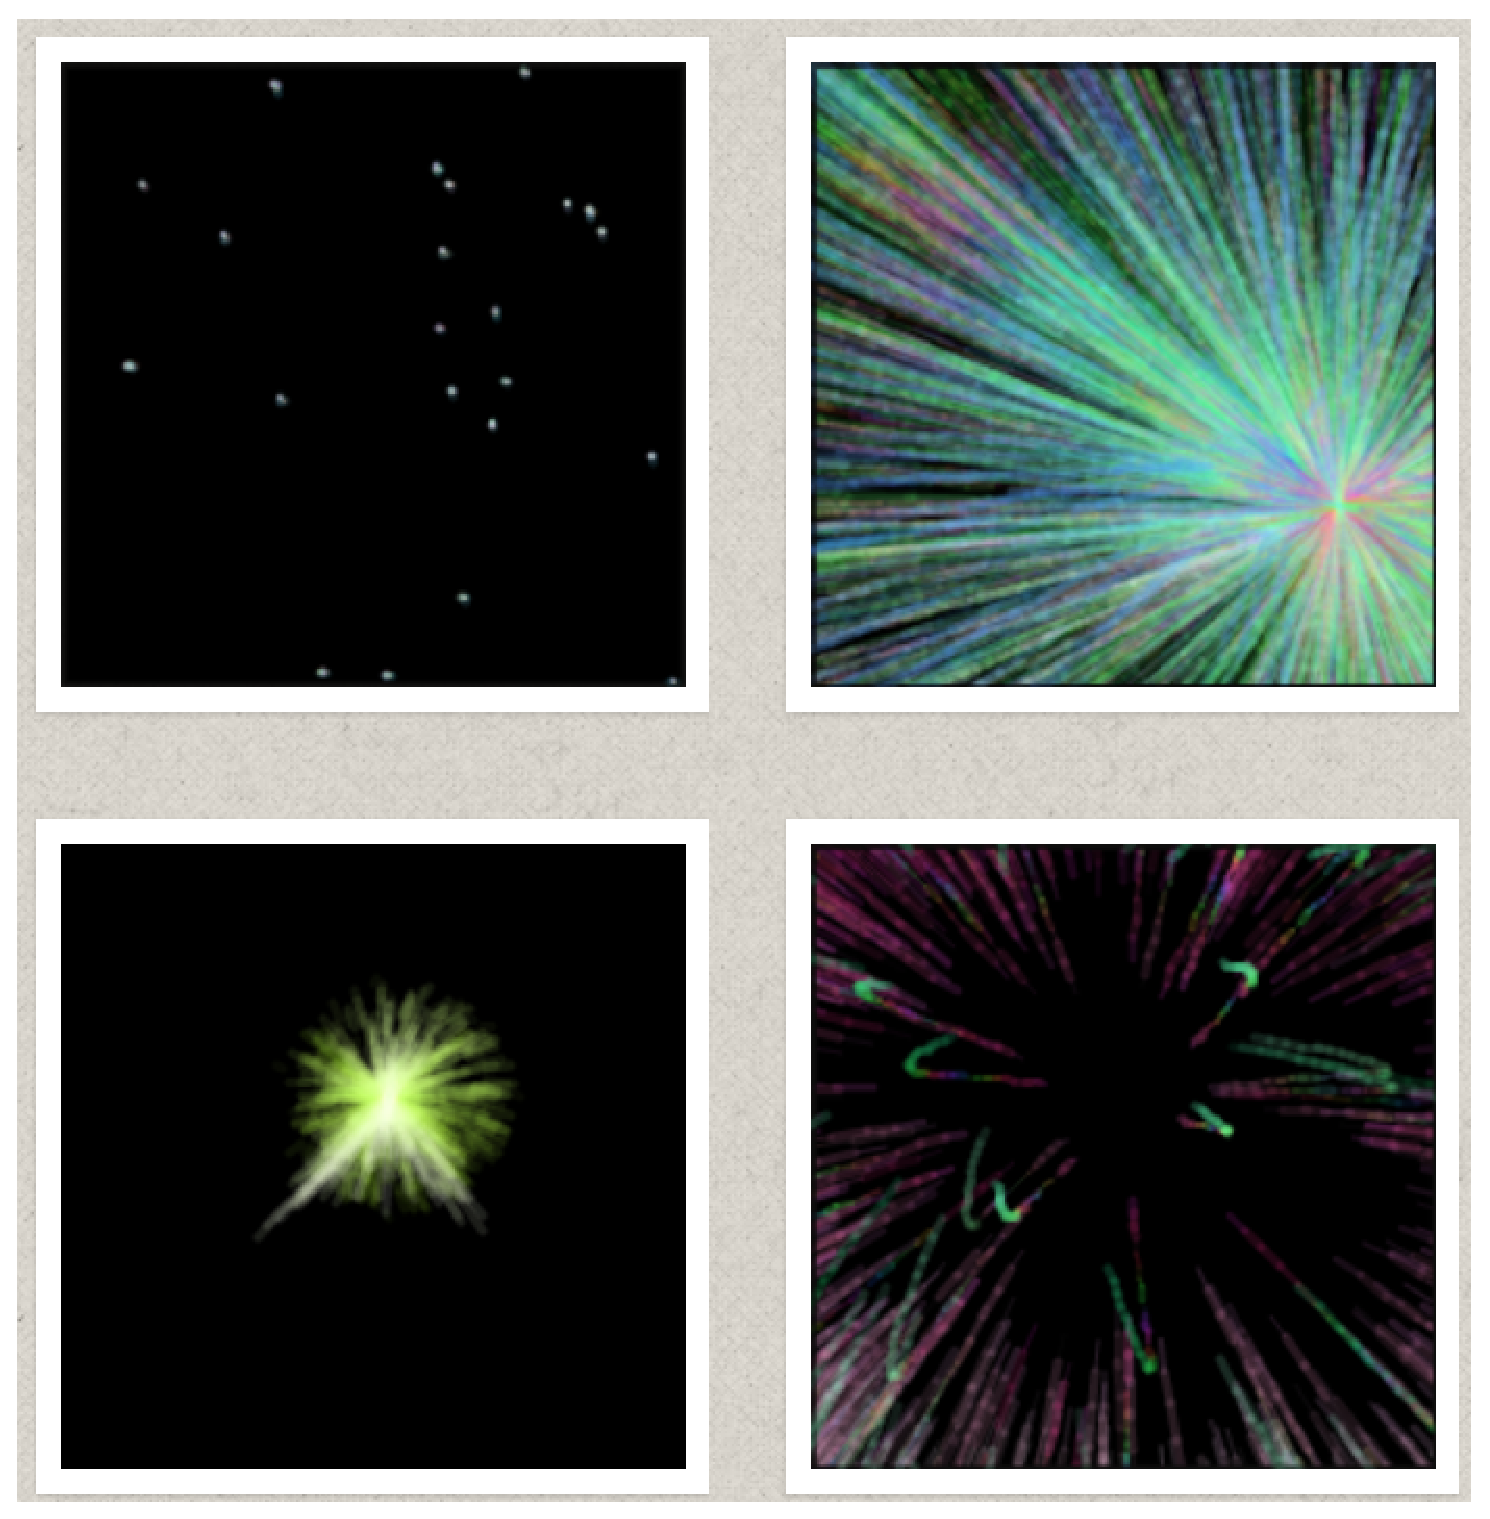
\includegraphics[width=8cm]{examples.eps}
    \caption{Snapshots of evolved individuals with the Fireworks application stored in the collection of a system user.}
    \label{fig:collection}
\end{figure}

\begin{figure}[t]
  \centering
  \subfigure[]
    {
\includegraphics[width=4cm]{1.eps}}
  \subfigure[]
    {
\includegraphics[width=4cm]{2.eps}}
  \subfigure[]
    {
\includegraphics[width=4cm]{3.eps}}
  \subfigure[]
    {
\includegraphics[width=4cm]{4.eps}}
  \subfigure[]
    {
\includegraphics[width=4cm]{5.eps}}
  \subfigure[]
    {
\includegraphics[width=4cm]{6.eps}}
  \caption{Sample frames of of an evolved animation.}
  \label{fig:sequence}
\end{figure}


\section{Concluding Remarks}
\label{sec:conclusions}
This paper presents a collaborative interactive evolutionary algorithm (C-IEA) developed on top of the EvoSpace platform.
The algorithm provides a store that hosts the evolving population, which can be accessed by remote clients over a web browser.
Connected clientes, called EvoWorkers, provide an interactive application to end users that evaluate the individuals produced by the algorithm.
Thus, fitness evaluation and genetic variations are carried out asynchronously over a distributed evolutionary process.
The algorithm is able to incorporate user collaboration by considering fitness evaluations provided by all connected users of the system.

The C-IEA application is called \emph{Fireworks}, that is designed to produce artistic animations of 3D particle swarms.
The animations are coded using the Processing programming language, that eases development for artists and other non-computer scientists,
that are more interested in the creative and artistic process.
Individuals are coded using a linear GP approach, that facilitates the representation of diverse particle behaviors, that give rise
to interesting patterns and displays.
The system continues to run and evolve in an open ended manner, continuously searching and evolving towards solutions that can better integrate
diverse user preferences.


%\section*{Acknowledgment}
%Funding for this work provided CONACYT (Mexico) Basic Science Research Project No. 178323
%and DGEST (Mexico) Research Project No. TIJ-ING-2012-110.
%This work was also supported by projects 4616.12-P and 4617.12-P awarded by DEGEST-ProIFOPEP (Mexico); TIN2011-28627-C04-03 and -02 (ANYSELF);
%awarded by the Spanish Ministry of Science and Innovation; P08-TIC-03903 (EvOrq) awarded by the Andalusian Regional Government; and project
%83 (CANUBE) awarded by the CEI-BioTIC UGR
%(\url{http://biotic.ugr.es}).

\bibliographystyle{IEEEtran}
\bibliography{biblio}



% that's all folks
\end{document}


